\documentclass[handout, xcolor=dvipsnames]{beamer}


\mode<presentation> {

\usetheme{Berlin}
\usetheme{Warsaw}

\setbeamertemplate{itemize items}[ball] % if you want a ball
\setbeamertemplate{itemize subitem}[circle] % if you wnat a circle
\setbeamertemplate{itemize subsubitem}[triangle] % if you want a triangle

\setbeamertemplate{blocks}[rounded][shadow=true]
\setbeamertemplate{navigation symbols}{}
\setbeamertemplate{mini frames}[square]
\setbeamersize{text margin left=6mm, text margin right=4mm}
\setbeamercolor{button}{bg = white, fg = blue}


\defbeamertemplate*{footline}{my theme}
 {
  \leavevmode%
  \hbox{%
  \begin{beamercolorbox}[wd=.35\paperwidth,ht=2.25ex,dp=1ex,center]{author in head/foot}%
    \usebeamerfont{author in head/foot}\insertshortauthor%~~(\insertshortinstitute USU)
  \end{beamercolorbox}%
  \begin{beamercolorbox}[wd=.65\paperwidth,ht=2.25ex,dp=1ex,center]{title in head/foot}%
    \usebeamerfont{title in head/foot}\insertshorttitle
  \end{beamercolorbox}%
  \begin{beamercolorbox}[wd=.1\paperwidth,ht=2.25ex,dp=1ex,right]{date in head/foot}%
     %\usebeamerfont{date in head/foot}\insertshortdate{}\hspace*{2em}
    %\insertframenumber{}\hspace*{2ex} 
  \end{beamercolorbox}}%
  \vskip0pt%
}

 % or ...

  \setbeamercovered{transparent}
  % or whatever (possibly just delete it)
}


\usetheme{Darmstadt}
\usefonttheme[onlylarge]{structurebold}
\setbeamerfont*{frametitle}{size=\normalsize,series=\bfseries}
\setbeamertemplate{navigation symbols}{}

\usepackage[english]{babel}
\usepackage{multirow}
\usepackage[latin1]{inputenc}
\usepackage{times}
\usepackage[T1]{fontenc}
\usepackage{graphicx}
\usepackage{natbib} %citep and citet
\usepackage{color}
\usepackage{amsmath}

%%% for references
\renewcommand{\bibsection}{\subsubsection*{\bibname}} % to avoid References creates new section/subsection in header
\bibpunct[:]{(}{)}{;}{a}{}{,}




\begin{document}

% here you define the information that will be displayed in the title/cover page

\title[\hspace*{0.5cm} Statistical Visualization II, Utah State University
	   \hspace*{80pt}\hfill \insertframenumber\hspace*{0.5cm}]
       {An Interactive Tool to Visualize Results from Uncertainty Quantification}


\author[\hspace*{0cm}Matt Isaac --- April 9, 2019\hspace*{0.25cm}]
		{Matt Isaac\\
		e-mail: \tt{matt.isaac@aggiemail.usu.edu} \\[-0.8cm]
		~ \\
		% \flushright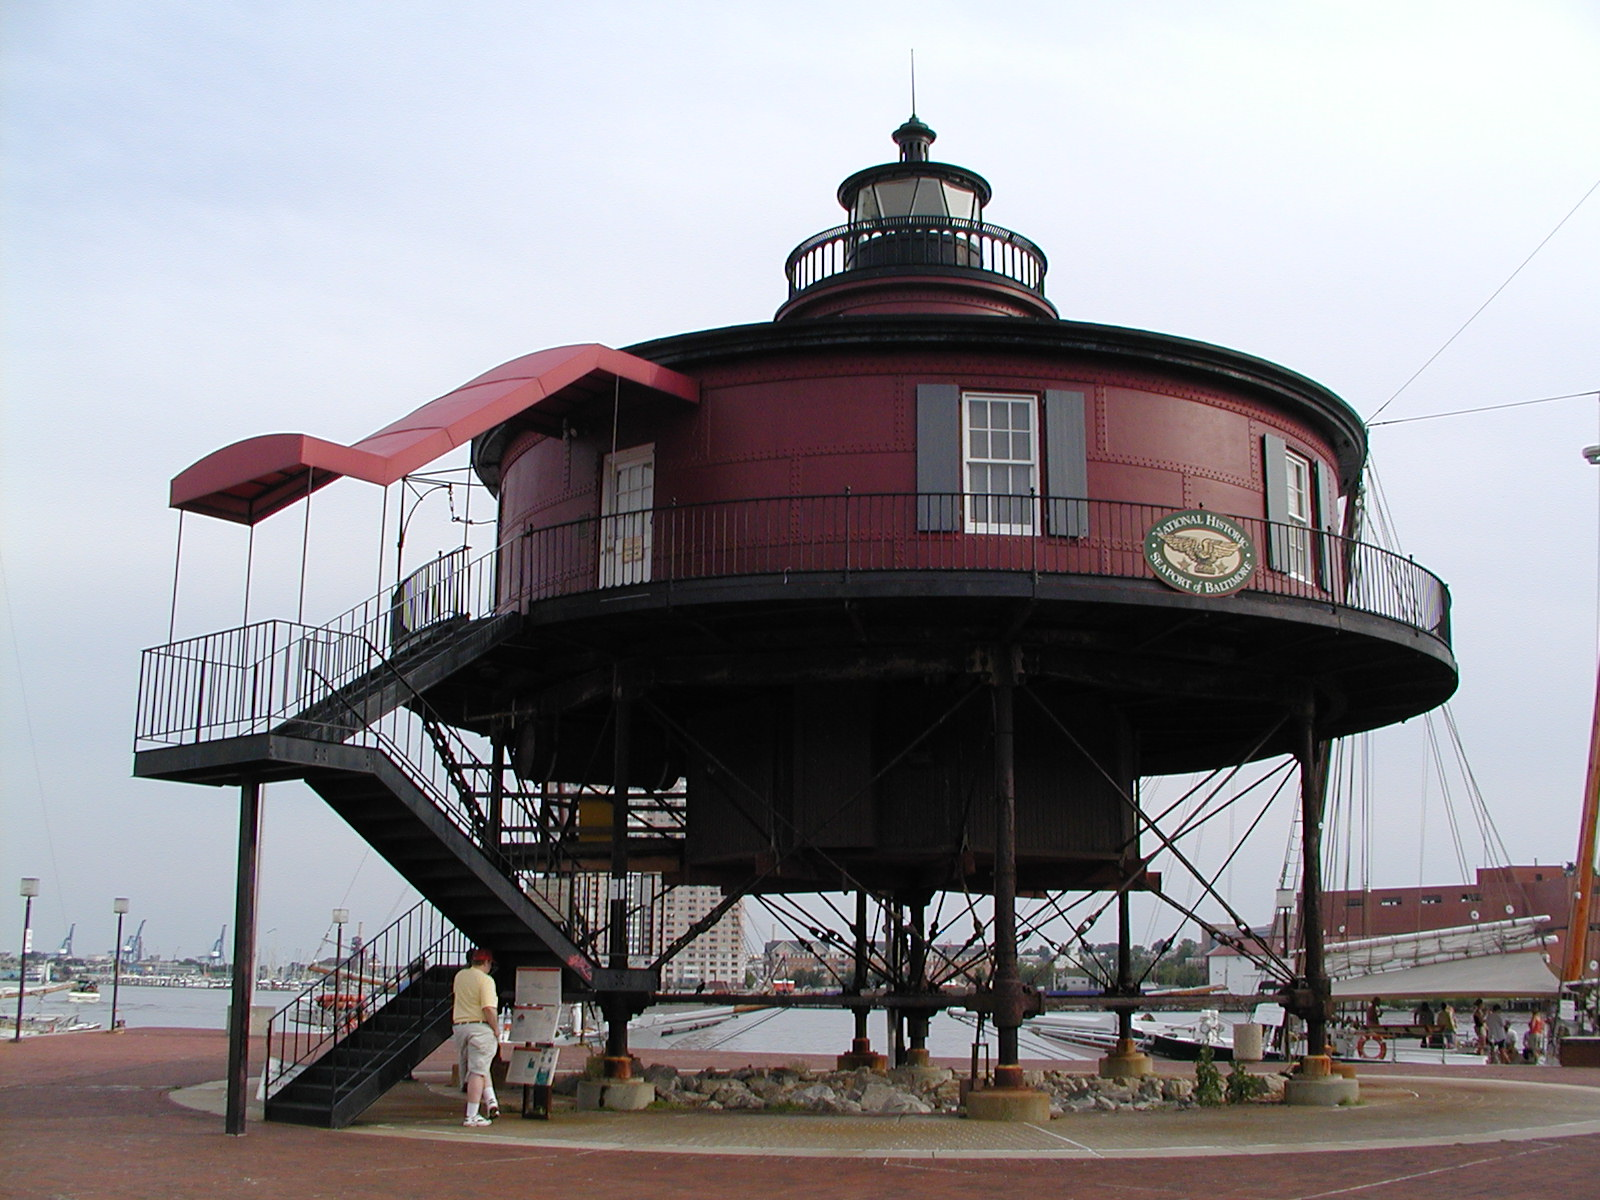
\includegraphics[height=2.0cm]{figures/Baltimore_P5260032}
		}


\date{April 9, 2019}


% here you build the title page
\frame{
  \titlepage
}


% outline 
\AtBeginSection[]
{
  \begin{frame}<beamer>{outline}
    \frametitle{Outline}
    \small
    \tableofcontents[currentsection]%,hideothersubsections]
    \normalsize
  \end{frame}
}


% If you wish to uncover everything in a step-wise fashion, uncomment
% the following command:

%\beamerdefaultoverlayspecification{<+->}


%%%%%%%%%%%%%%%%%%%%%%%%%
%%%   Outline           %
%%%%%%%%%%%%%%%%%%%%%%%%%

\begin{frame} 
\frametitle{Outline}
  \tableofcontents
  % You might wish to add the option [pausesections]
\end{frame}

\newcounter{finalframe}

%%%%%%%%%%%%%%%%%%%%%%%%%
\section{Introduction}  
%%%%%%%%%%%%%%%%%%%%%%%%%

\subsection{}
\begin{frame}
	\frametitle{Motivation}
	Uncertainty Quantification (UQ):
	\begin{itemize}
    	\item Is a branch of simulation analysis that is used often in engineering contexts; 
    	\item Assists engineers and decision-makers in finding a balance between design efficiency and design sufficiency (avoid under/over designing);
    	\item Provides a quantification of how variability in a system can influence the end state of that system. 
    \end{itemize}
\end{frame}


\subsection{}
\begin{frame}
	\frametitle{UQ Overview - Terminology}
	\begin{description}
		\item[aleatory uncertainty:] Uncertainty resulting from randomness inherent to a given parameter. Gaining more knowledge about the parameter will not reduce the uncertainty of the parameter. 
	  \item[epistemic uncertainty:] Uncertainty resulting from a lack of knowledge about a given parameter. Gaining more knowledge about the parameter could reduce the uncertainty of the parameter. 
	  \item[engineering model:] A mathematical model that defines the relationship between the parameters (model inputs) and SRQ (model output). 
	  \item[system response quantity (SRQ):] A parameter of particular interest directly related to the engineering system in question. The SRQ is the output (i.e. prediction) from the engineering model.

	\end{description}
\end{frame}


\begin{frame}
	\frametitle{UQ Overview - Algorithm}
	\[\text{Aleatory model inputs: }A_k, k = 1, 2, 3 \]
	\[\text{Epistemic model inputs: }E_k, k = 1, 2, 3\]
	\[ SRQ = E_1^{E_2}A_3A_2^{A_1} + E_3\]
	\\
	\begin{itemize}
	\item Probability distributions for each input is selected by subject matter expert
	\end{itemize}	
	\begin{center}
	{\scriptsize Example adapted from \cite{EW2018}}
	\end{center}
\end{frame}

\begin{frame}
	\frametitle{UQ Overview - Algorithm}
	\begin{center}
	\begin{center} 
	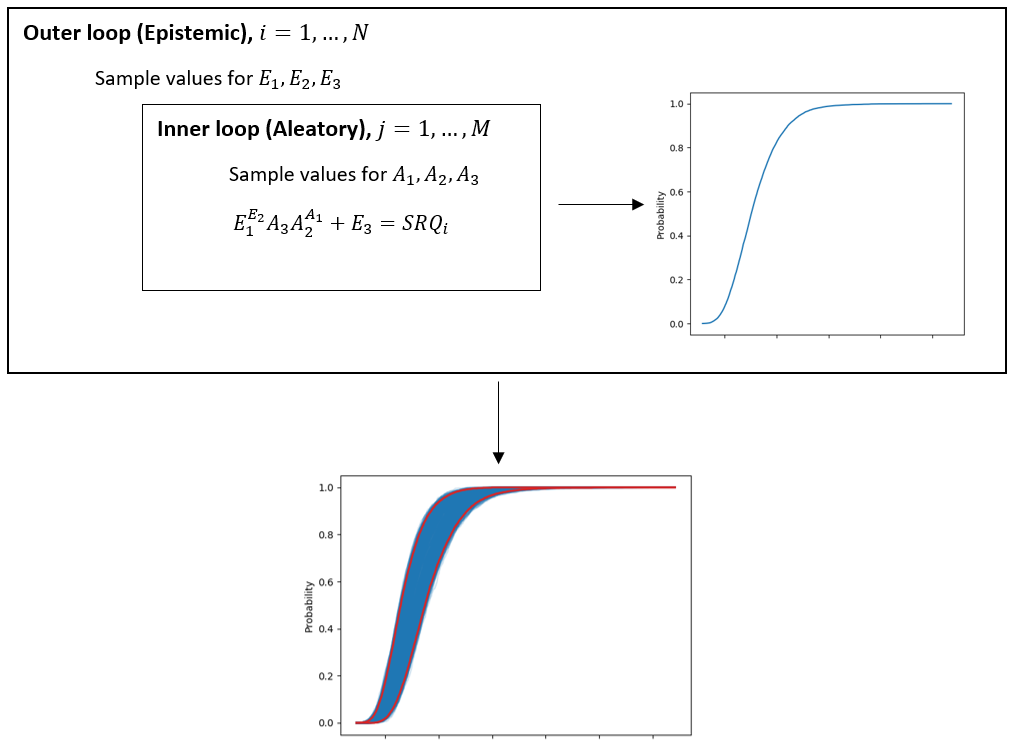
\includegraphics[height=6cm,width=7.5cm]{figures/uq_algo.png}
	\end{center}	
	{\scriptsize Diagram adapted from \cite{EW2018}}
	\end{center}
\end{frame}

\begin{frame}
	\frametitle{Project Goal}
	\textbf{Goal:} Develop an interactive tool to create meaningful visualizations (like the one below) and useful interpretations of results from a UQ simulation.\\
	\begin{center}
	\begin{center} 
	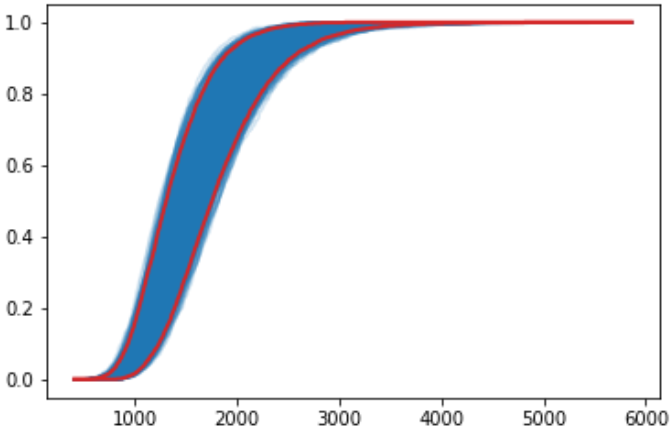
\includegraphics[height=4cm,width=5cm]{figures/viz_exmp.png}
	\end{center}	
	\end{center}
\end{frame}

%%%%%%%%%%%%%%%%%%%%%%%%%
\section{Methods}  
%%%%%%%%%%%%%%%%%%%%%%%%%

\subsection{}
\begin{frame}
	\frametitle{Key Features}
		\begin{itemize}
		\setlength\itemsep{1.5em}
		\item upload data via a {\tt .csv} file
		\item toggle P-box and CDF's on/off
		\item select upper/lower percentiles to be used in P-box calculation
		\item adjustable transparency for CDF ensemble
		\item extract either a probability interval or an SRQ interval from P-box
		\item download and save visualization as a {\tt .png} file
    \end{itemize}
\end{frame}

\begin{frame}
	\frametitle{Planned Layout}
	\begin{center}
	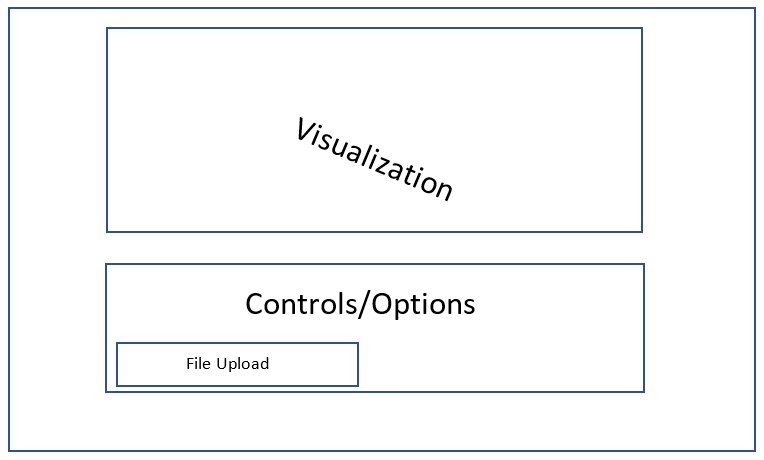
\includegraphics[height=7cm,width=11cm]{figures/proto_app_layout.png}
	\end{center}	
\end{frame}

\subsection{}
\begin{frame}
	\frametitle{{\tt R} Packages}
	\begin{description}[labelwidth=4em]

\item[{\bf dplyr:}] {\footnotesize The {\tt dplyr} package \citep{DPLYR} was used for data wrangling and data manipulation}

\item[{\bf shiny:}] {\footnotesize The {\tt shiny} package \citep{SHINY} provided the framework on which the application was developed and deployed. It also contains the implementations for all user-interface components (toggle buttons, check boxes, numeric inputs, sliders, etc.).}

\item[{\bf shinydashboard:}] {\footnotesize The {\tt shinydashboard} package \citep{DASH} was used as a wrapper around the {\tt shiny} framework to give a clean, polished appearance to the application.}

\item[{\bf ggplot2:}] {\footnotesize The plotting functionality of the {\tt ggplot2} package \citep{GGPLOT} was used to generate the actual visualization and to add, remove, or adjust components on the plot.}

\end{description}
\end{frame}


%%%%%%%%%%%%%%%%%%%%%%%%%
\section{Results}  
%%%%%%%%%%%%%%%%%%%%%%%%%

\subsection{}
\begin{frame}
	\frametitle{Deployment}
	\begin{center} 
		Shiny App currently deployed at: \\ {\tt https://misaac.shinyapps.io/UQViz/}
	\end{center}
\end{frame}

\subsection{}
\begin{frame}
	\frametitle{Data Source}
	\begin{itemize}
	\item Users can upload {\tt .csv} files for visualization. The files should have the x values in the 1st column, and the CDFs in subsequent columns. 
	\item For convenience, a sample data set is also provided
	\end{itemize}
	\begin{center} 
		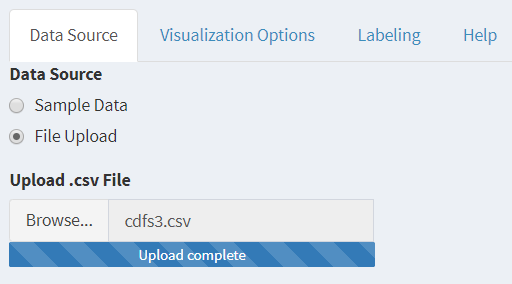
\includegraphics[height=3cm,width=6cm]{figures/tab_ds.png}
	\end{center}
\end{frame}

\subsection{}
\begin{frame}
	\frametitle{Visualization Options}
	\begin{itemize}
	\item Several options are provided to allow customized visualizations 
	\end{itemize}
	\begin{center} 
		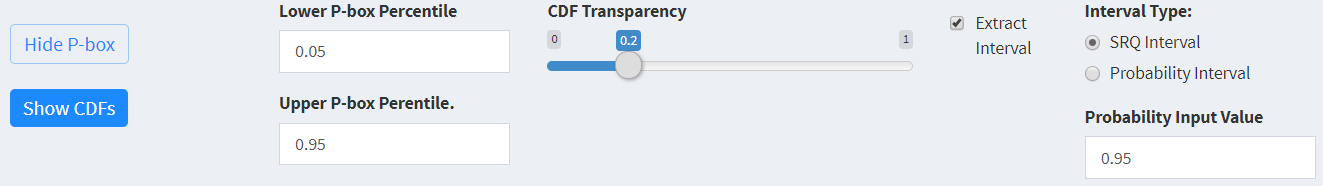
\includegraphics[height=2.25cm,width=11cm]{figures/tab_vo.png}
	\end{center}
\end{frame}

\subsection{}
\begin{frame}
	\frametitle{Visualization Options}
	\begin{center} 
		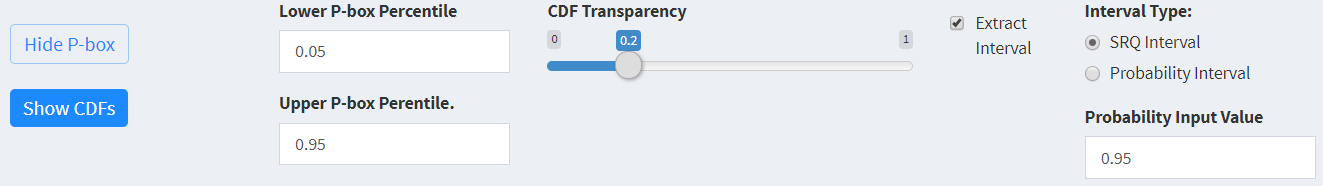
\includegraphics[height=2.25cm,width=11cm]{figures/tab_vo.png}
	\end{center}
	\begin{figure}
	  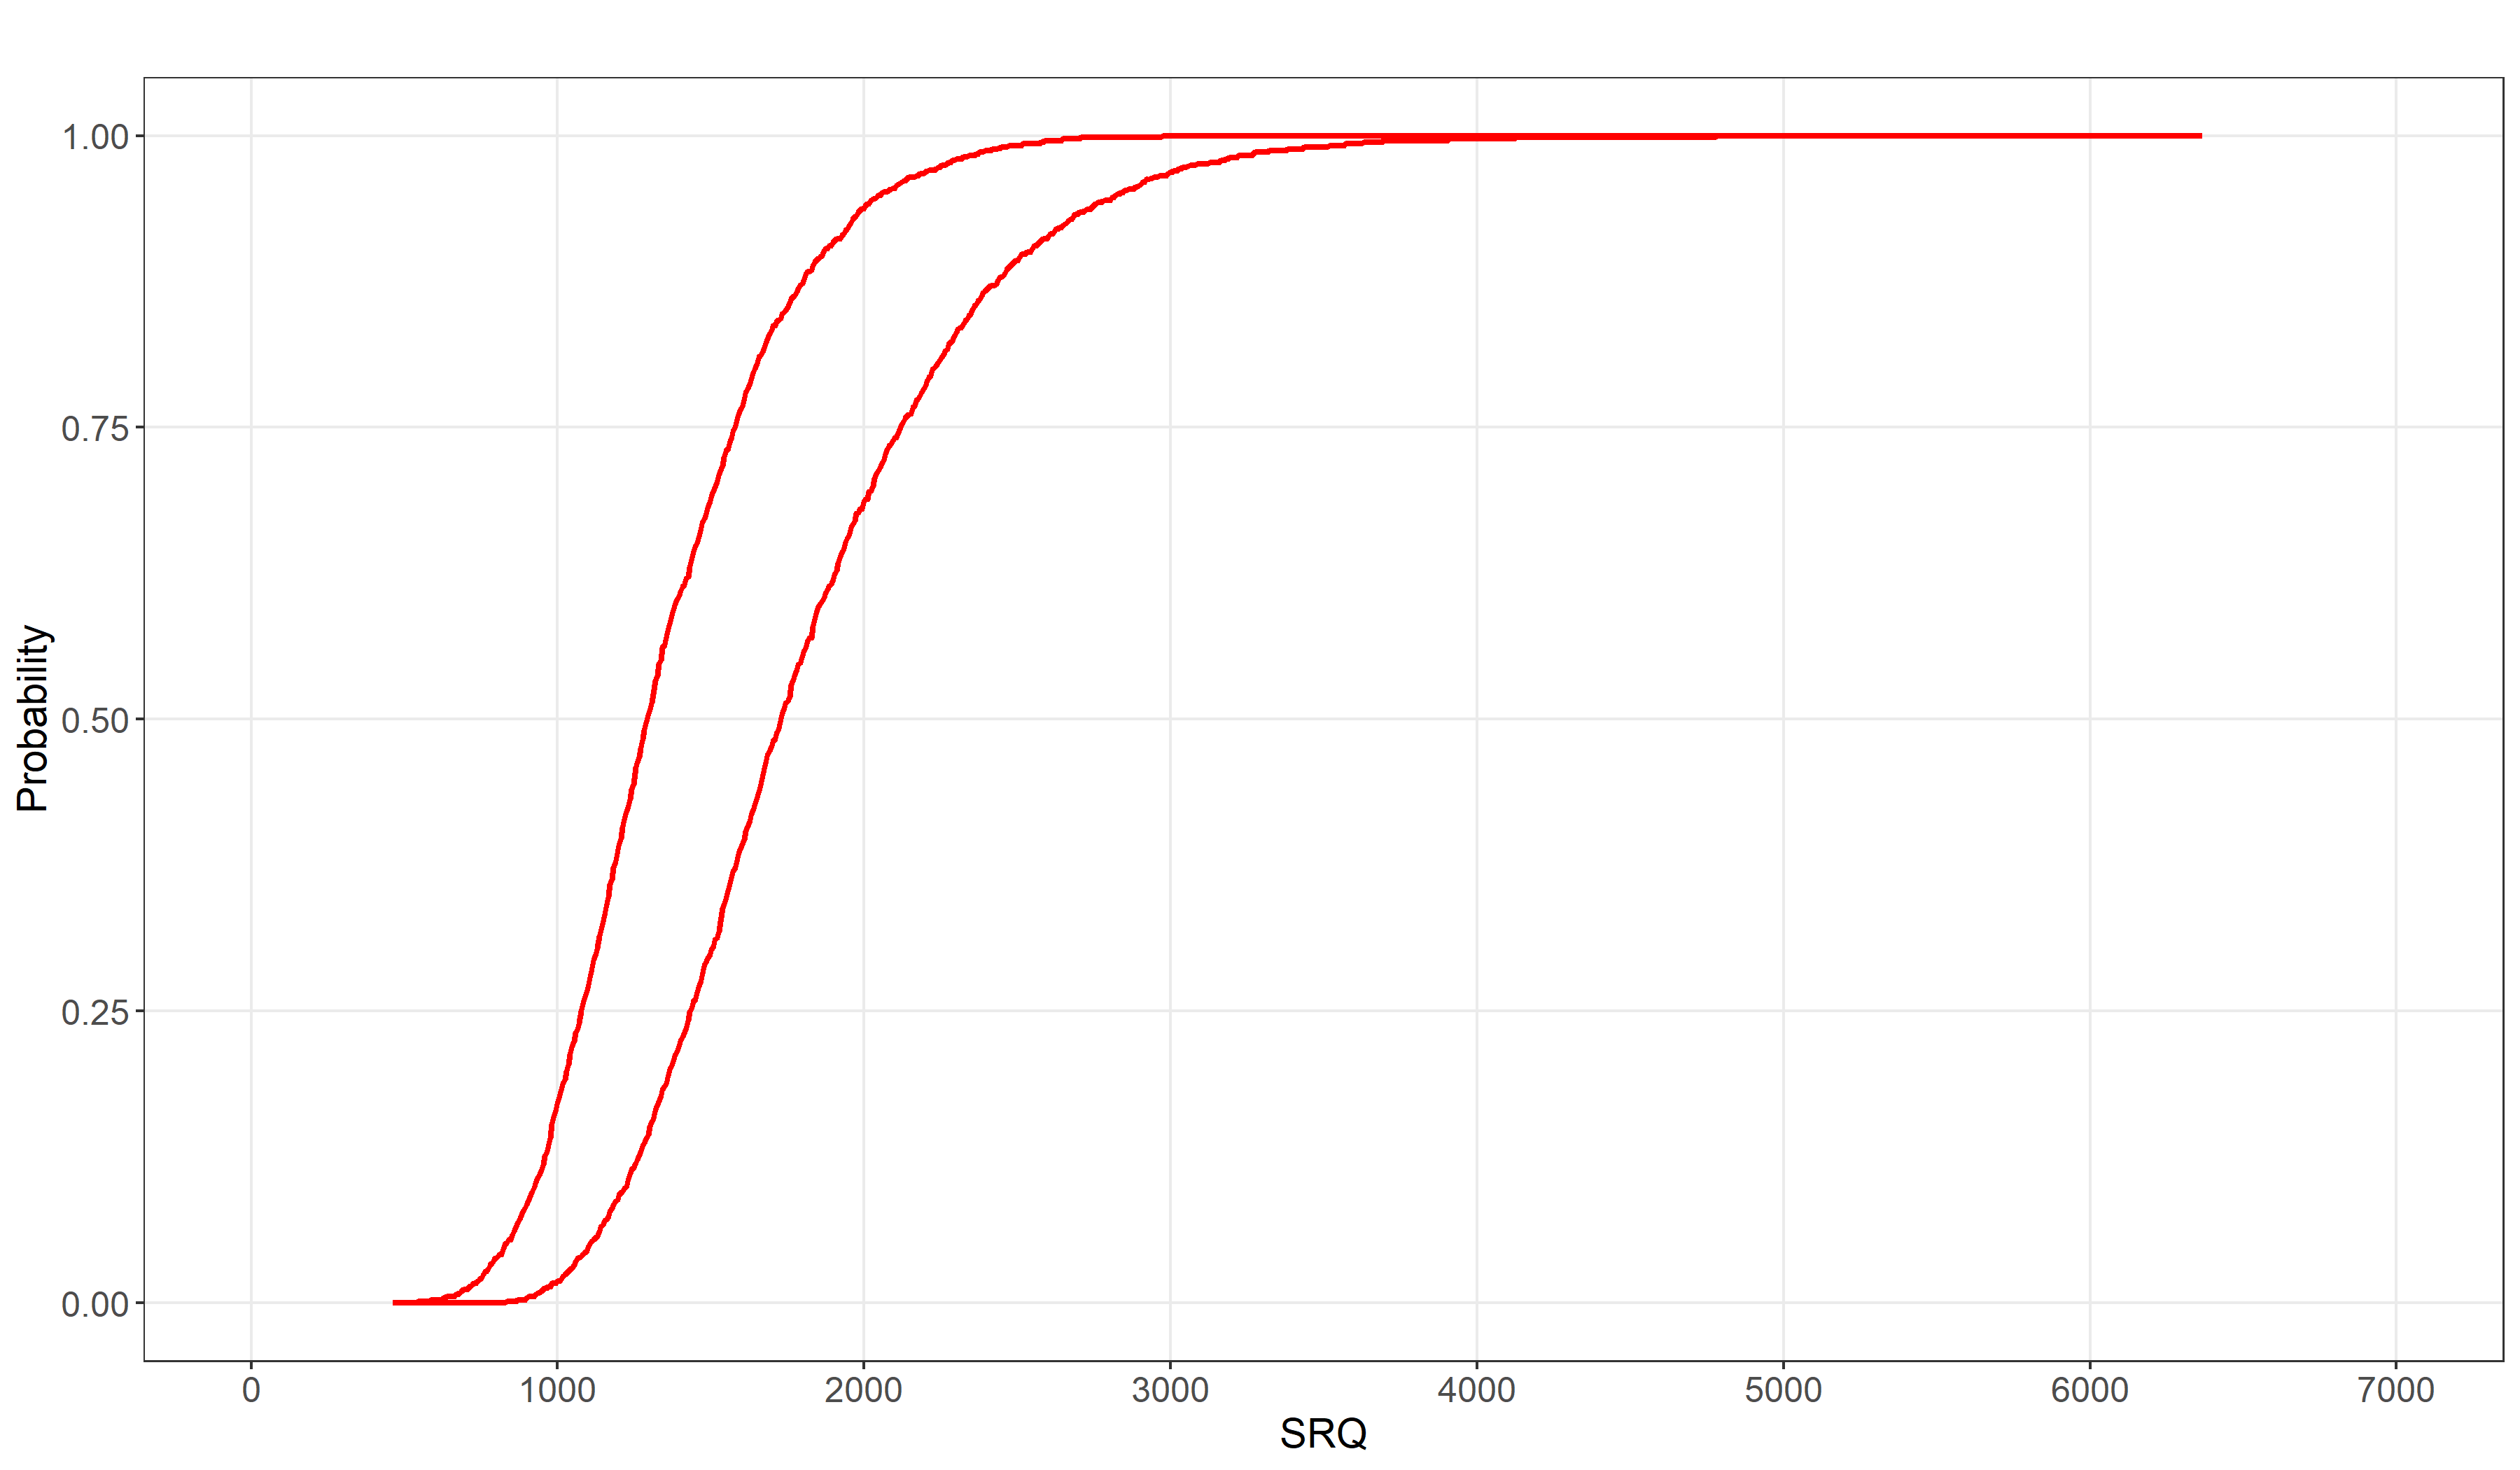
\includegraphics[height=3cm,width=3.5cm]{figures/pbx.png}
	  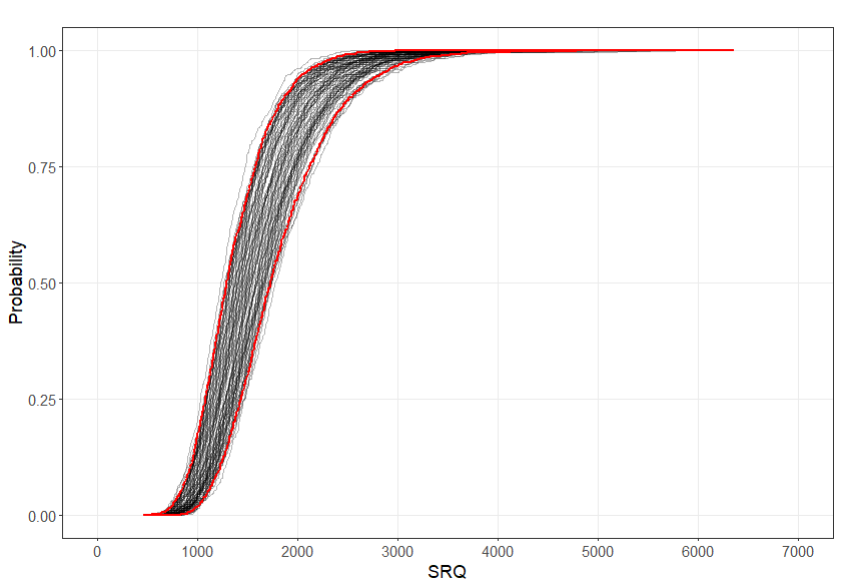
\includegraphics[height=3cm,width=3.5cm]{figures/pbx_cdf_l.png}
	  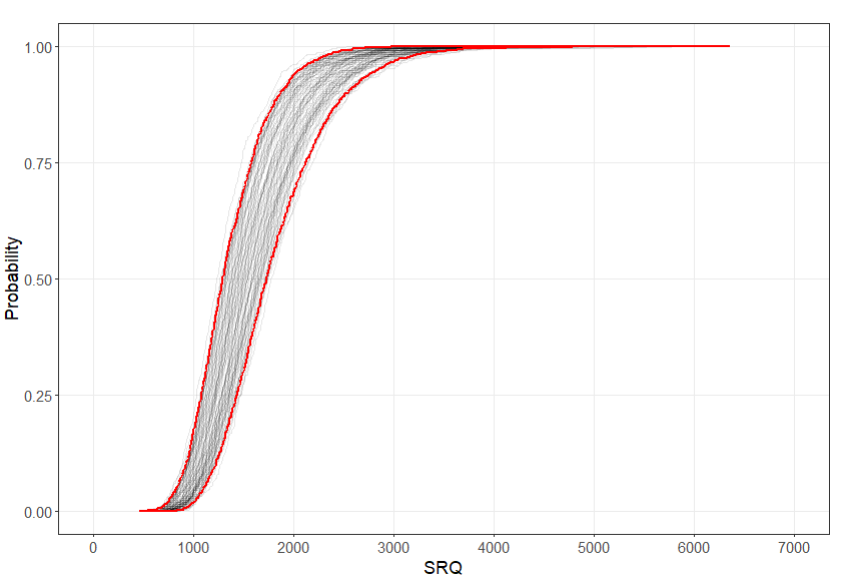
\includegraphics[height=3cm,width=3.5cm]{figures/pbx_cdf_d.png}
	\end{figure}
\end{frame}

\subsection{}
\begin{frame}
	\frametitle{Labeling}
	\begin{itemize}
	\item Custom title and x-axis label can be added to adapt visualization to domain. 
	\end{itemize}
	\begin{center} 
		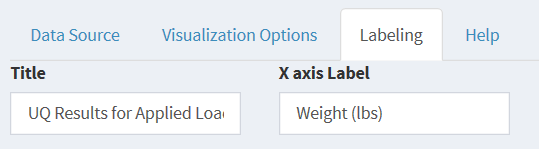
\includegraphics[height=1.5cm,width=5.5cm]{figures/tab_lb.png} \\
		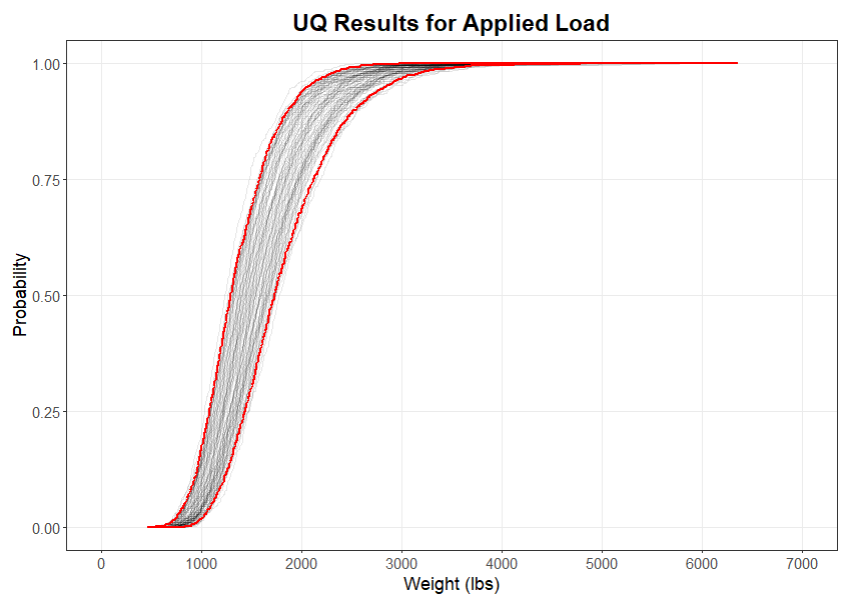
\includegraphics[height=4cm, width=6cm]{figures/plt_labeled.png}
	\end{center}
\end{frame}

\subsection{}
\begin{frame}
	\frametitle{Interpretation - Extract Probability or SRQ Intervals}
  There are two ways a P-box can be used for interpretation:
	\begin{itemize}
	  \item{Input SRQ value to extract probability interval}
	  \item{Input probability value to extract SRQ interval}
	\end{itemize}
\end{frame}

\subsection{}
\begin{frame}
  \frametitle{Interpretation - Extract Probability Interval}
  \begin{center}
    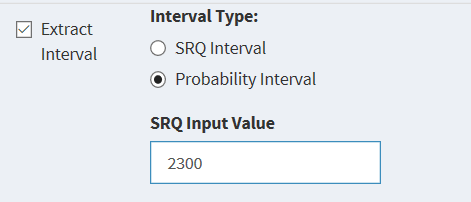
\includegraphics[height=1.25cm, width=3.25cm]{figures/prob_int_ctrl.png} \\
    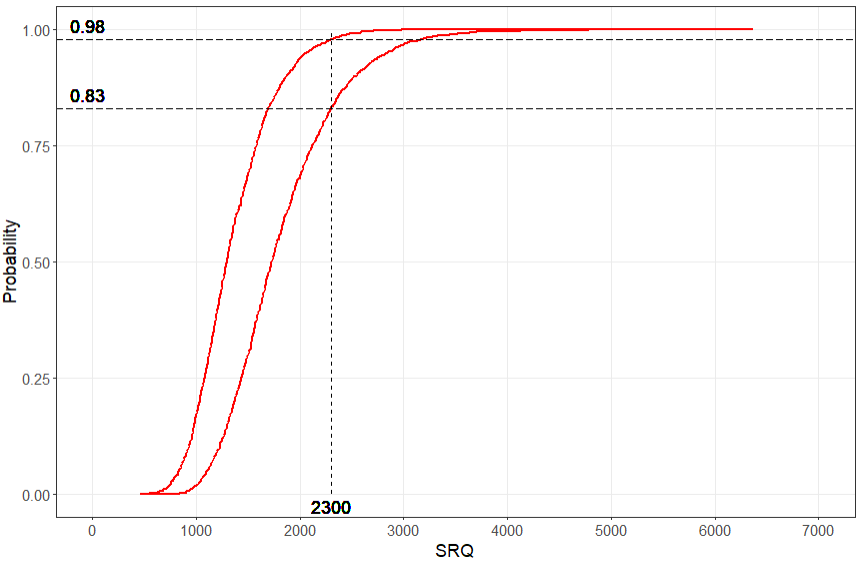
\includegraphics[height=5.75cm, width=8cm]{figures/prob_int.png}
  \end{center}
\end{frame}

\subsection{}
\begin{frame}
  \frametitle{Interpretation - Extract SRQ Interval}
  \begin{center}
    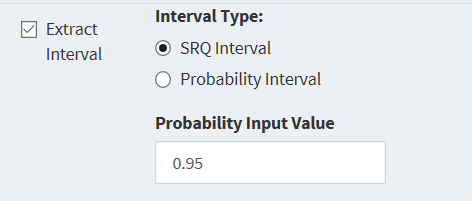
\includegraphics[height=1.25cm, width=3.25cm]{figures/srq_int_ctrl.png} \\
    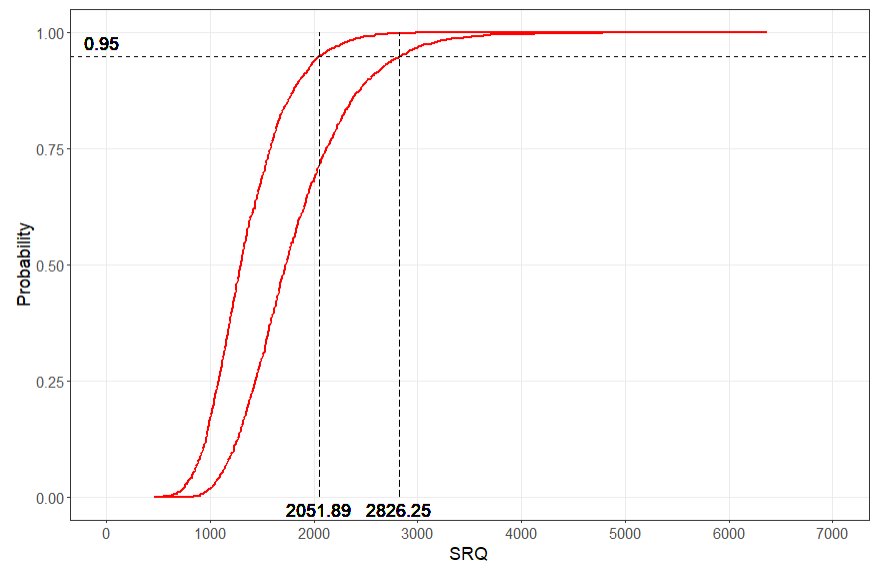
\includegraphics[height=5.75cm, width=8.25cm]{figures/srq_int.png}
  \end{center}
\end{frame}

%%%%%%%%%%%%%%%%%%%%%%%%%
\section{Discussion}  
%%%%%%%%%%%%%%%%%%%%%%%%%

\subsection{}
\begin{frame}
  \frametitle{Challenges}
  \begin{itemize}
    \item{Long render time for hundereds (or thousands!) of traces on a plot}
    \item{File upload size limit to {\tt shiny} web applications}
  \end{itemize}
\end{frame}

\subsection{}
\begin{frame}
  \frametitle{Future Work}
    \begin{itemize}
      \item{Create a self contained UQ simulation tool -- perform entire process, start to finish}
      \begin{itemize}
        \item{Choose an SRQ function}
        \item{Define inputs as aleatory or epistemic}
        \item{Specify the number of inner and outer loop iterations}
        \item{Visualization generated automatically}
      \end{itemize}
    \end{itemize}
\end{frame}
      
\subsection{}
\begin{frame}
	\frametitle{}
	\begin{center}
  {\large \bf Questions ??} --- \\[1cm]
    or e-mail: \tt{matt.isaac@aggiemail.usu.edu}
  \end{center}
\end{frame}

\subsection{}
\begin{frame}
	\frametitle{Sources}

	\bibliographystyle{elsarticle-harv}
	
  {\footnotesize
	\bibliography{references2}}


\end{frame}


\end{document}

